%% Condensed from dissertacao-en/chapters/cap5-benchmark.tex @295dde3.
\chapter{The Multi-Criteria Benchmark}
\label{chap:benchmark}

This chapter answers RQ1 with the 250-cell matrix (14 models
$\times$ 18 datasets; two structural exclusions) measured under
Chapter~\ref{chap:metodologia}'s protocol. The reading is in two
movements: within the 11-model core --- the roster defined by order
of entry into the study, prior to the 2026 extension --- the top of
binary-classification accuracy is a statistical tie; the 2026
generation then shifts the top without that tie ever being rejected.
Full per-act syntheses, secondary metrics and disaggregated tables
are in the extended report and appendix.

\section{The statistical tie of the 11-model core}
\label{sec:cap5-ato1}
\label{sec:cap5-ato4}

On the 10 binary datasets, the Friedman test rejects rank
homogeneity ($\chi^2 = 31.3$, $p = 5.2\times10^{-4}$;
Iman--Davenport $F = 4.1$), but the Nemenyi post-hoc separates
almost nothing: with $k{=}11$ and $N{=}10$ the critical distance is
4.77, and the top bar connects TabPFN (mean rank 3.2) to the MLP
(Figure~\ref{fig:cap5-cd}). The equivalence reading therefore comes
from the Bayesian signed-rank instrument with a region of practical
equivalence of one percentage point of AUC: under the lenient
criterion ($E[\theta] > 0.5$), \textbf{8 of the 10} non-leading
models are practically equivalent to the leader --- itself already a
foundation model, TabPFN; under the strict criterion (posterior mass
of equivalence above 0.95), \textbf{3 of the 10}: XGBoost (0.999),
LightGBM (0.992) and CatBoost (0.957). The criteria were fixed after
the analysis began and are reported as a sensitivity sweep: ROPE
radii $0.005/0.01/0.02$ give $2/8/10$ equivalents under the lenient
criterion and $0/3/5$ under the strict one --- the conclusion holds
for ROPE $\geq 0.01$. Variance decomposition completes the picture:
families explain $\eta^2 = 0.20$ and models-within-family $0.11$ of
rank variance (together 0.31), leaving 0.69 to the
dataset-interaction-plus-noise term --- the winner depends more on
the dataset than on the family, and ``boosting always wins'' finds
no margin in accuracy. Figure~\ref{fig:cap5-heatmap} shows the full
primary-metric matrix with within-dataset ranks as color.

\begin{figure}[htb]
\centering
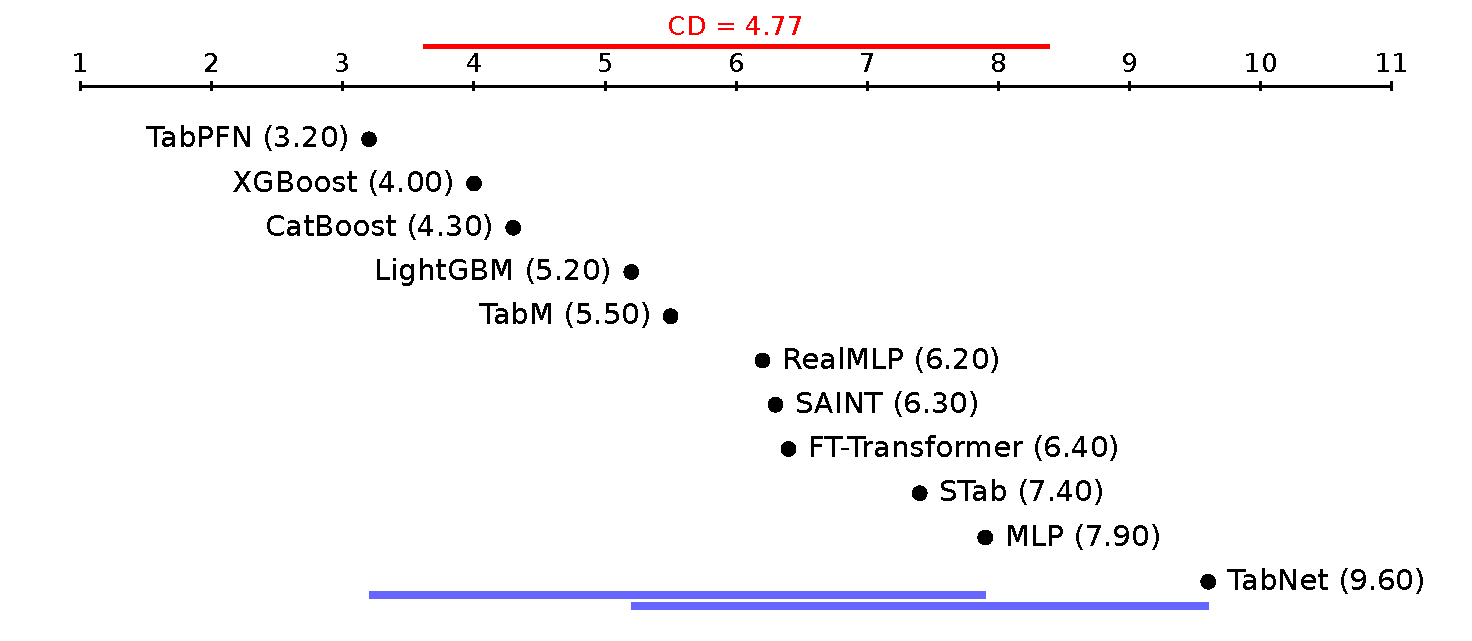
\includegraphics[width=0.9\linewidth]{images/cd_diagram_binary_11.pdf}
\caption[Critical-difference diagram, 11-model core]{Nemenyi
critical-difference diagram for binary classification on the
11-model core ($N{=}10$, $\mathrm{CD}=4.77$). The top bar connects
TabPFN to the MLP: the post-hoc does not separate the pack, which is
why the equivalence reading uses the Bayesian instrument.}
\label{fig:cap5-cd}
\end{figure}

\begin{figure}[htb]
\centering
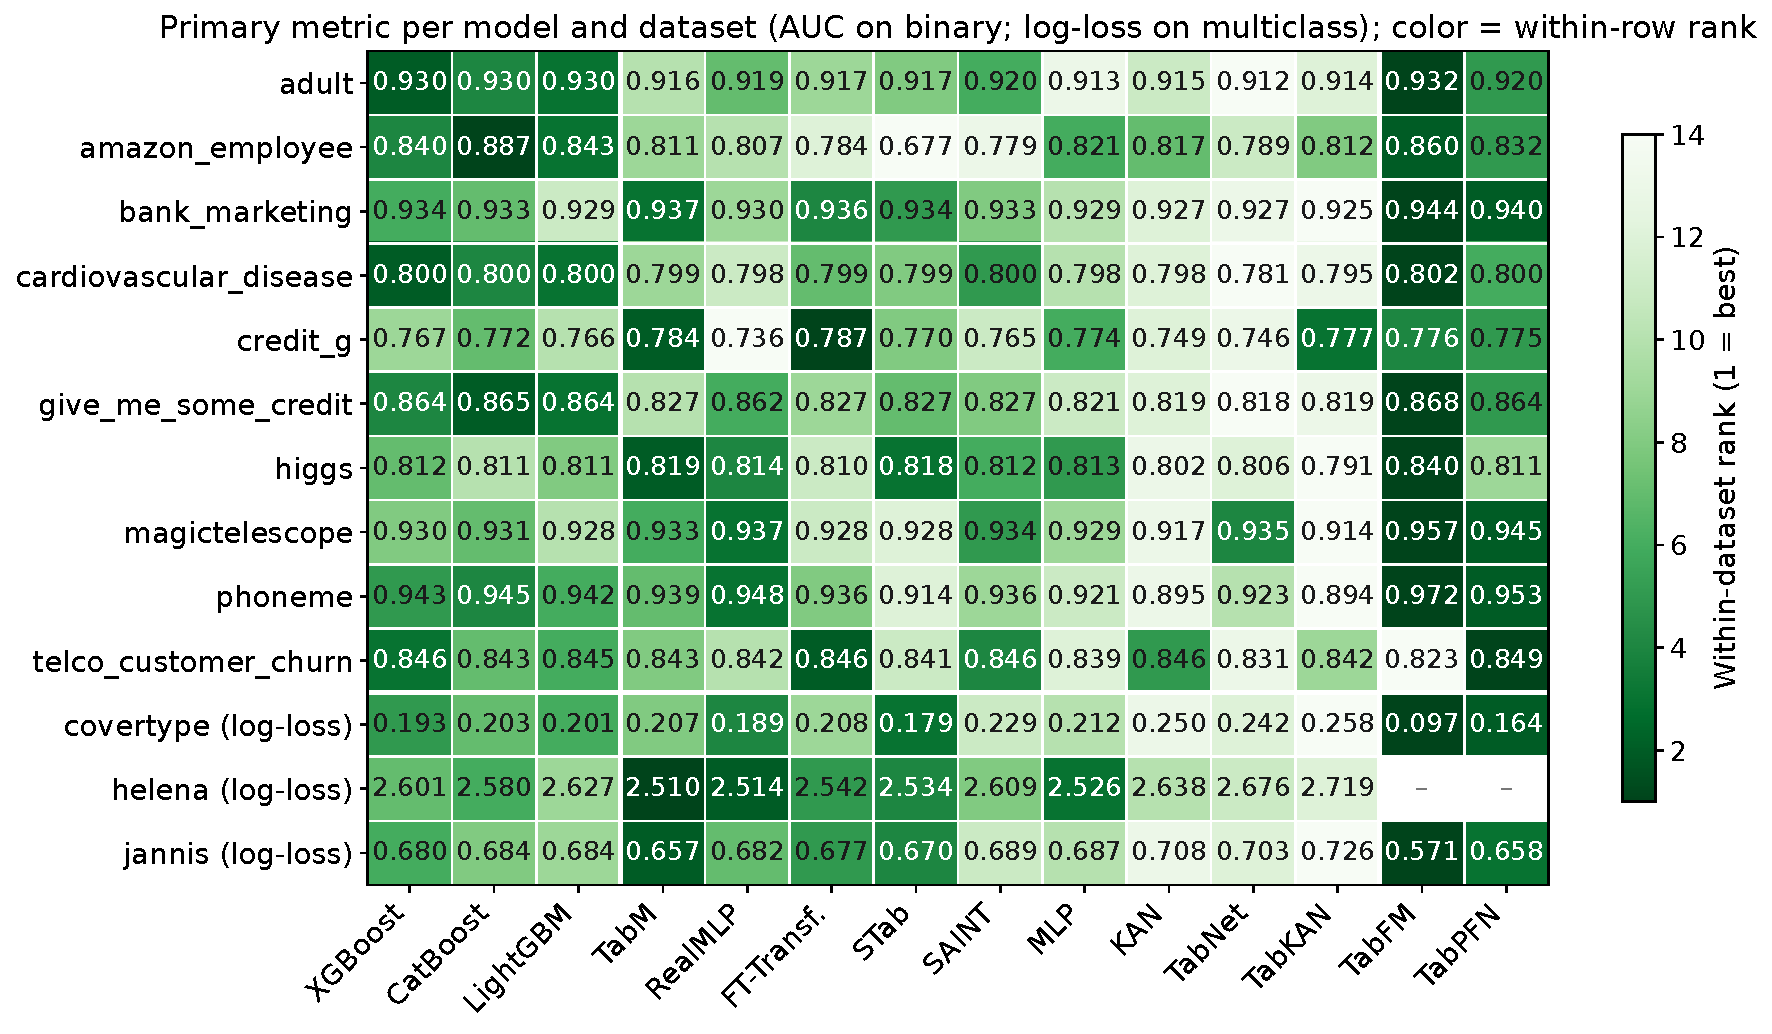
\includegraphics[width=\linewidth]{images/heatmap_classification_en.pdf}
\caption[Primary metric per model and dataset]{Primary metric per
model and classification dataset (AUC on binary, log-loss on
multiclass); color encodes the within-dataset rank (darker =
better). Empty cells: structural exclusions
(\texttt{helena}~$\times$~FMs).}
\label{fig:cap5-heatmap}
\end{figure}

\section{Cost axes: training, tuning, latency}
\label{sec:cap5-custos}

Accuracy near-ties make cost the deciding axis.
\textbf{Training}: median fit time over the 18 datasets --- 17 for
TabPFN --- spans ${\sim}300\times$ (LightGBM 0.66~s, XGBoost 0.69~s,
TabPFN 1.35~s at one forward pass, against ${\sim}200$~s for
SAINT/STab-class deep models). \textbf{Tuning}: GBDTs complete their
100-trial search in 104--646~s; deep models pay up to 14{,}622~s
(STab) --- a $140\times$ spread --- while the in-context models pay
zero by construction. \textbf{Inference latency} (amortized batch,
each model on its natural device, measured on \texttt{adult}):
XGBoost serves at 0.33~\us/row, TabPFN at 7{,}416, TabFM at 43{,}262
--- about five orders of magnitude for TabFM
($\approx131{,}000\times$), with the ratio varying by dataset
(full per-model costs in the appendix).
Figure~\ref{fig:cap5-pareto} folds accuracy and cost into Pareto
fronts: on the core, \{TabPFN, XGBoost, LightGBM\} on the
training-cost axis, narrowing to \{XGBoost, TabPFN\} on latency; on
the full grid the front becomes \{XGBoost, TabPFN, TabFM\}, with the
foundation models paying four to five orders of magnitude of latency
for the rank.

\begin{figure}[htb]
\centering
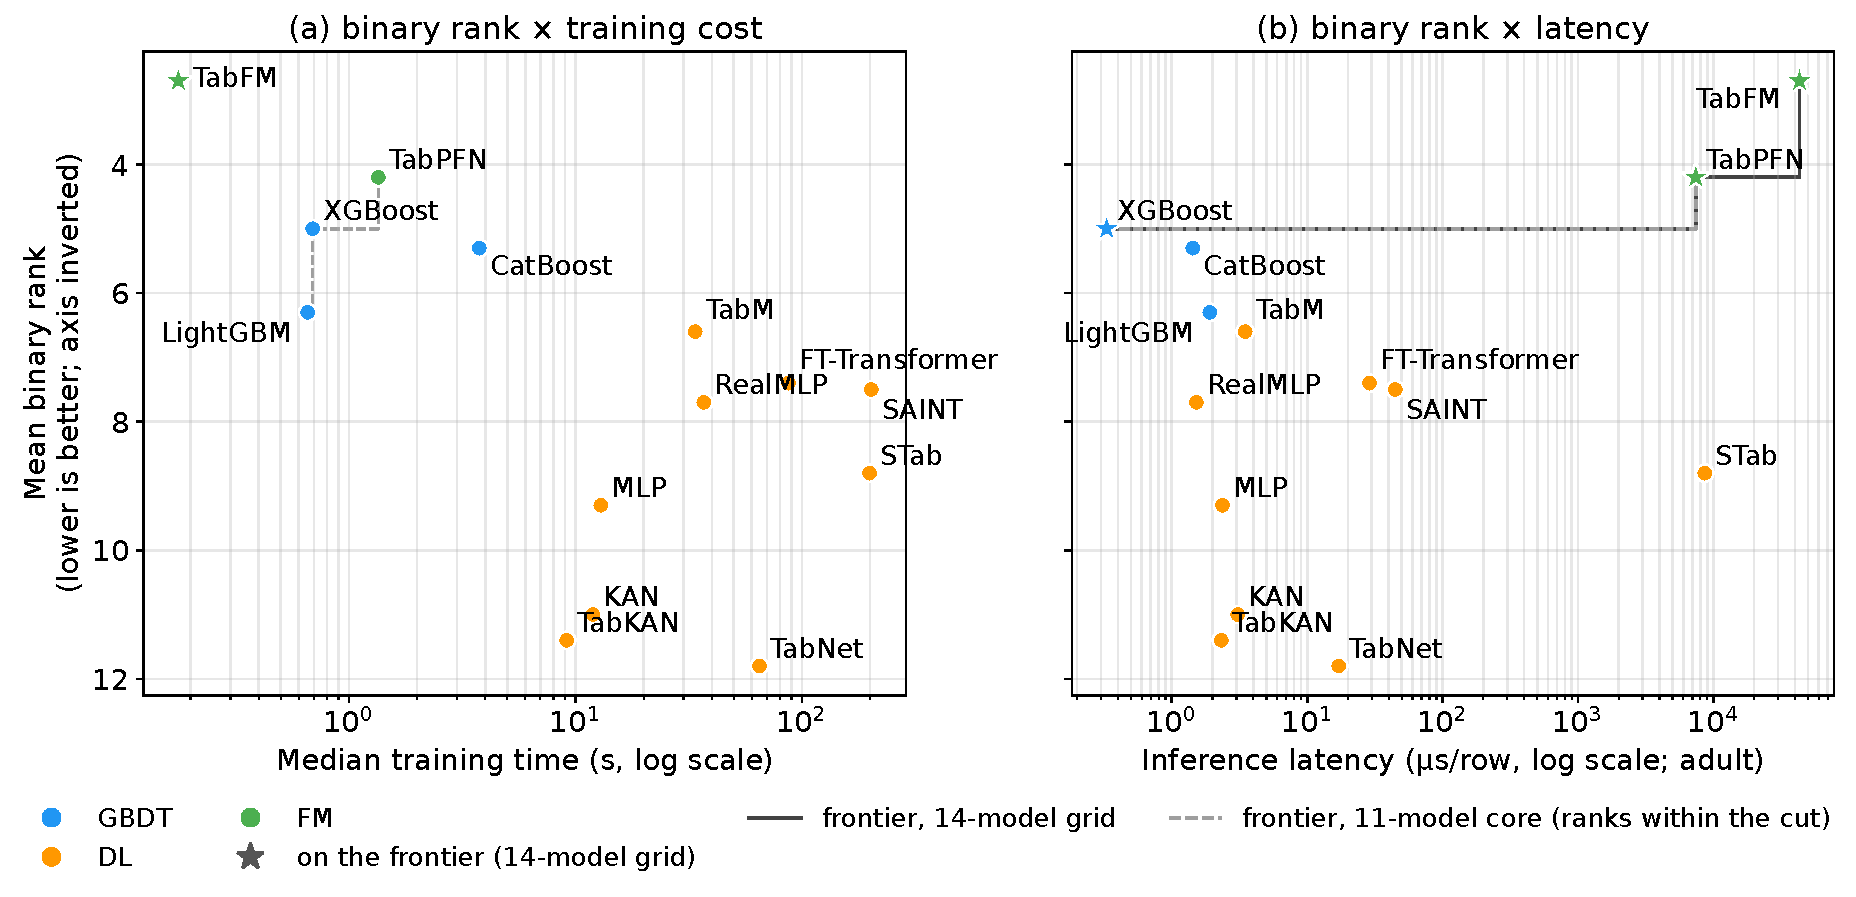
\includegraphics[width=\linewidth]{images/pareto_binary_en.pdf}
\caption[Accuracy--cost Pareto fronts]{Mean binary rank against
median training time (left) and inference latency (right), full
14-model grid; stars mark the Pareto front.}
\label{fig:cap5-pareto}
\end{figure}

\section{Conditional reversals: imbalance and sample size}
\label{sec:cap5-reversals}

Leadership is conditional on regime. Under class imbalance the GBDTs
\emph{gain} ground as severity grows (mean rank 6.6 in the mild
band, 5.5 moderate, 4.6 severe) while tabular deep learning loses it
(8.7/8.9/9.6); the foundation models stay ahead in every band
(3.3/4.1/2.7). On the sample-size axis, learning curves on five
datasets (500 samples to the full pool,
Figure~\ref{fig:cap5-curvas}) show the GBDT$\leftrightarrow$DL
crossover is real and dataset-specific --- deep learning overtakes
for good on 3 of 5 (2 of 4 setting aside
\texttt{year\_\allowbreak prediction}, whose DL curves reflect the
unstandardized target), while on \texttt{adult} the GBDT takes the
lead at $n \approx 4{,}000$ --- and TabPFN has the best
regime-averaged metric on all five swept datasets for
$n \leq 4{,}000$: the zero-shot paradigm is strongest exactly where
data are scarce.

\begin{figure}[htb]
\centering
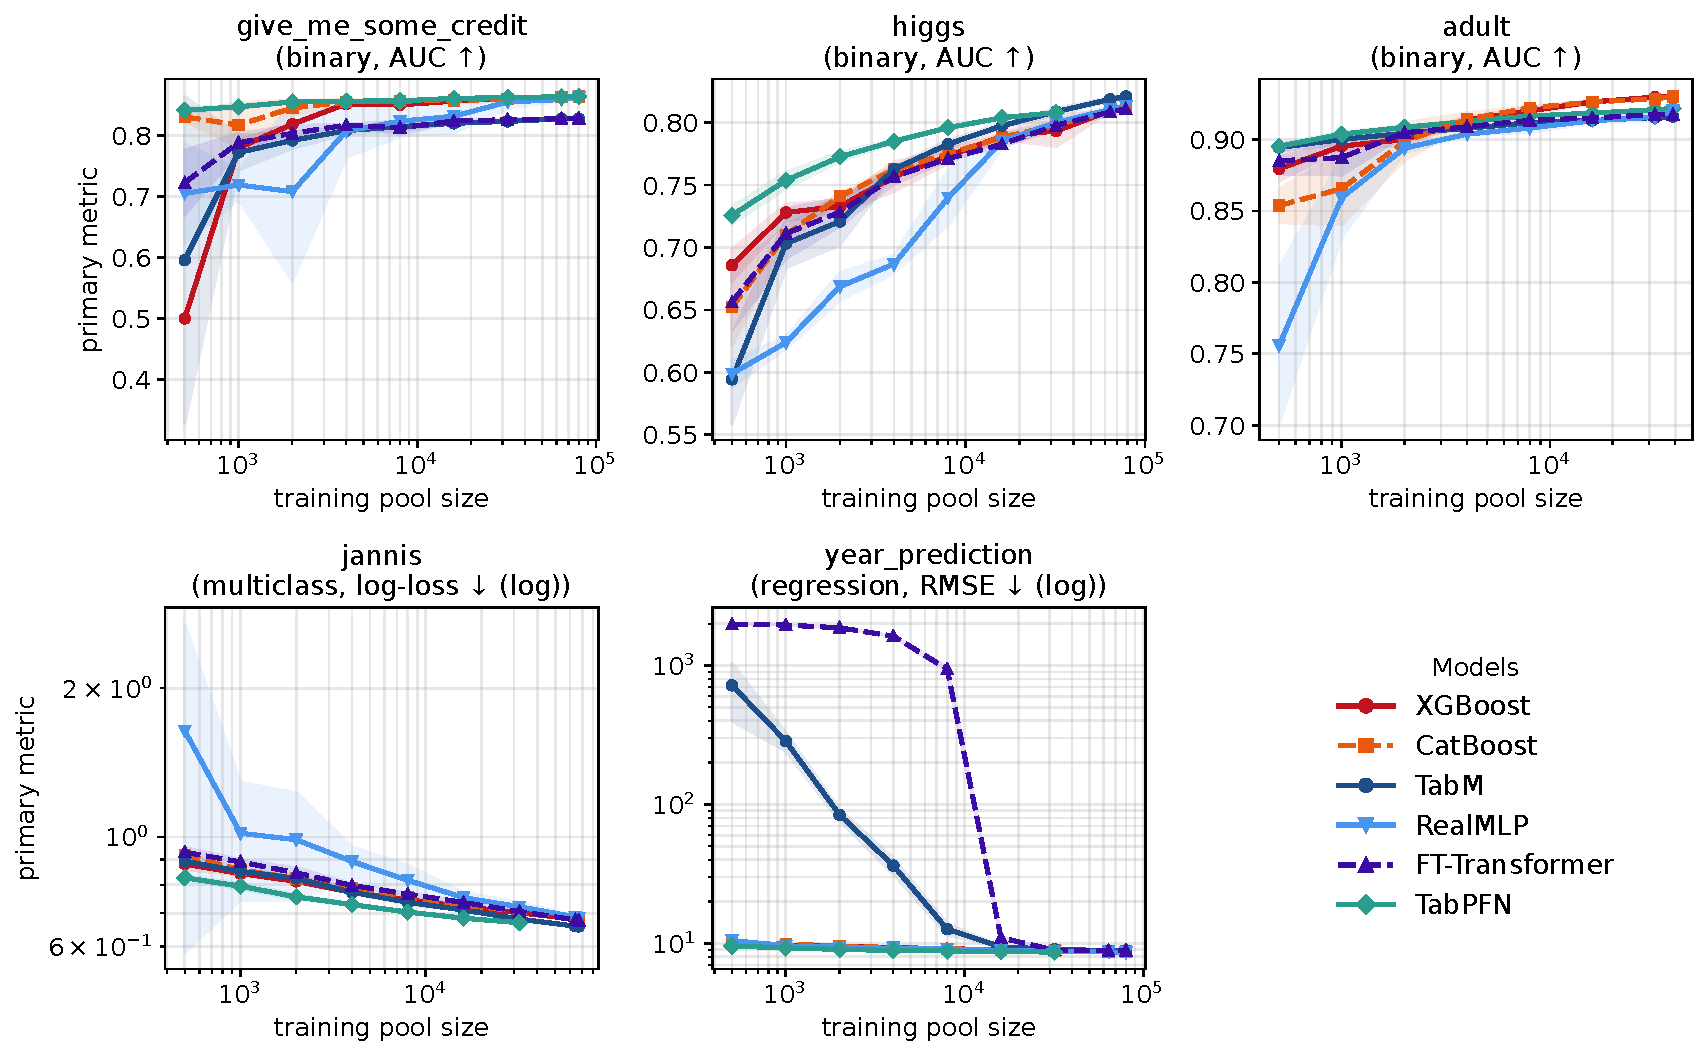
\includegraphics[width=\linewidth]{images/learning_curves_diss_en.pdf}
\caption[Learning curves on five datasets]{Primary metric against
training-set size (log), five datasets $\times$ six models, 3 seeds
(bands: $\pm1$ sd). The last panel carries the legend.}
\label{fig:cap5-curvas}
\end{figure}

\section{The 2026 generation shifts the top}
\label{sec:cap5-shift}

Extending the grid with the 2026 entrants (TabFM; KAN and TabKAN as
the Kolmogorov--Arnold representatives) changes the leadership
without rejecting the tie. Zero-shot TabFM leads the mean rank in
all three tasks (Table~\ref{tab:cap5-ranks}; in multiclass, over the
two datasets where it operates --- \texttt{helena}'s 100 classes are
a structural exclusion for both FMs) and is the single best model on
13 of the 18 datasets (operating on 17). The lead is consistent
across datasets, but no test confirms it as a statistical
separation: with $k{=}14$ the critical distance grows to 6.27 and
the underpowered post-hoc separates nothing; the paired effect size
against XGBoost is $d = 0.68$; and the Bayesian instrument puts 0.67
of the posterior on TabFM's superiority over XGBoost (0.33 on
equivalence; $E[\theta] = 0.40$), with equivalence modal against
CatBoost. In regression, $N{=}5$ puts the Wilcoxon floor at 0.0625
--- a combinatorial floor; multiclass ($N{=}3$) and regression
readings are descriptive. The Kolmogorov--Arnold family lands in the
bottom third on every task (KAN 11.0/12.0/9.8; TabKAN
11.4/13.3/11.8, behind even TabNet in multiclass and regression) ---
an informative negative, with the caveat that both are
reimplementations under a uniform protocol.

\begin{table}[htb]
\centering
\caption[Mean ranks per task, full grid]{Mean rank per task on the
full 14-model grid (lower is better; multiclass over the datasets
each model runs on). Full 14-row table in the extended report.}
\label{tab:cap5-ranks}
\begin{tabular}{lccc}
\toprule
 & Binary & Multiclass & Regression \\
\midrule
\textbf{TabFM}      & \textbf{2.7} & \textbf{1.00} & \textbf{1.2} \\
TabPFN              & 4.2          & 2.50          & 3.0 \\
Best non-FM         & XGBoost 5.0  & STab/TabM 3.67 & XGBoost 5.0 \\
KAN                 & 11.0         & 12.0          & 9.8 \\
TabKAN              & 11.4         & 13.3          & 11.8 \\
\bottomrule
\end{tabular}
\end{table}

\section{Instance-level complementarity}
\label{sec:cap5-ato5}

Where do the foundation models and XGBoost disagree? A sanity gate
first reproduces the benchmark's cells from stored predictions (52
cells, 51 exact and 1 within $6\times10^{-6}$), then per-instance
agreement is measured on the classification hold-outs: the FMs and
XGBoost agree on 93.6--95.0\% of instances, leaving a disputed
\emph{fringe} of 0.6--15.5\% per dataset. Inside the fringe the
asymmetry is strong and dataset-dependent: McNemar rejects the tie
at 1\% in 14 of 24 model$\times$dataset cells, with a median balance
of $+6.6$ net FM wins per 1{,}000 instances
(Figure~\ref{fig:cap5-compl}); TabFM converts the fringe
overwhelmingly on some datasets and \emph{loses} it on
\texttt{telco\_\allowbreak customer\_\allowbreak churn} --- the
dataset where Chapter~\ref{chap:metodologia}'s declared
preprocessing idiosyncrasy penalizes only the FM (0.8233 raw against
0.8515 with numeric \texttt{TotalCharges}), so that cell reads as a
pipeline artifact, not a model property. The two registered
mechanistic hypotheses are not confirmed at 5\%: FM gains
concentrate in minority-class instances on 7/10 datasets ($p=0.17$)
and in low-XGBoost-confidence instances on 8/10 ($p=0.055$). On
\texttt{amazon\_\allowbreak employee} (5.8\% minority) the practical
reading is sharp: near-identical accuracies (${\sim}94.3\%$) hide
minority recalls of 0.032 (XGBoost), 0.214 (TabPFN) and 0.298
(TabFM) at the 0.5 threshold --- when the minority class is what the
application pays for, the FMs' advantage is operational, not
cosmetic.

\begin{figure}[htb]
\centering
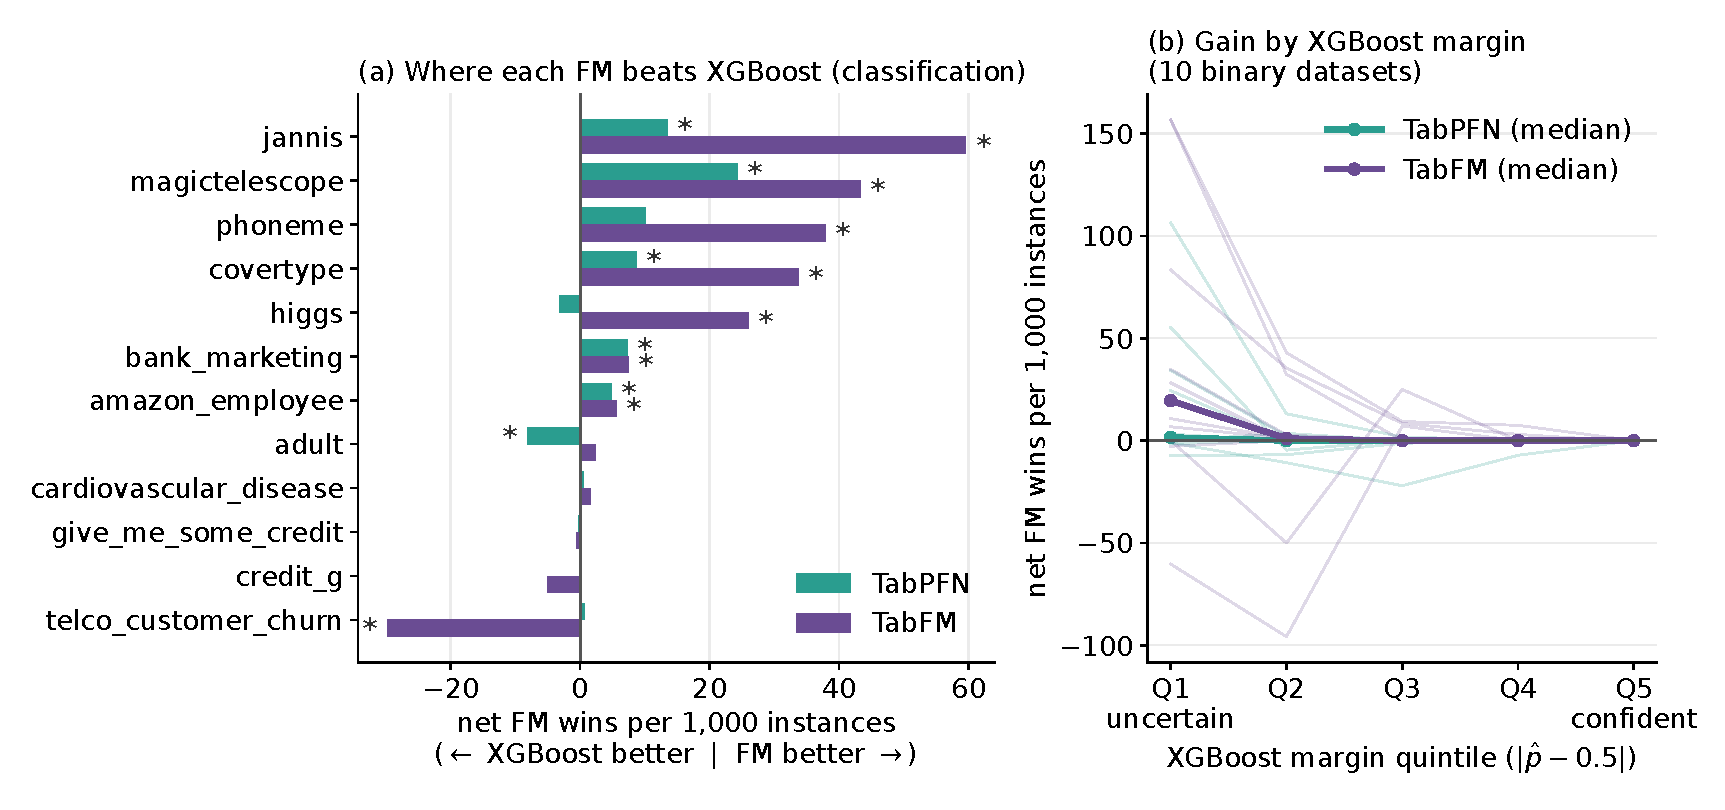
\includegraphics[width=\linewidth]{images/complementarity_diss_en.pdf}
\caption[Instance-level complementarity]{Net FM wins per 1{,}000
instances against XGBoost per dataset (left; $*$ = McNemar at 1\%)
and gain by XGBoost-margin quintile (right).}
\label{fig:cap5-compl}
\end{figure}

\section{Summary: the answer to RQ1}
\label{sec:cap5-sintese}

\emph{Within the pre-2026 core, the top of binary accuracy is a
statistical tie that includes a foundation model as leader; costs,
not accuracy, separate the models. The 2026 generation shifts the
top --- TabFM leads every task's mean rank and wins 13 of 18
datasets zero-shot --- without that tie ever being rejected by an
underpowered post-hoc or by the Bayesian instrument, and at the
price of about five orders of magnitude of serving latency on the
reference dataset. Leadership is conditional (imbalance, sample
size), and the per-instance layer shows where the FM advantage is
operational. The practical question moves from ``which family wins''
to ``which constraints decide'' --- Chapter~\ref{chap:framework}.}
